\chapter{Model 5: Ridge Regression}\label{ch:model5}

% Include the dynamic values from model calibration
% Model 5 Actual Values
% Generated: 2025-10-15 13:36:08

\renewcommand{\ModelFiveRSquaredTrain}{0.4940}
\renewcommand{\ModelFiveRSquaredTest}{0.4772}
\renewcommand{\ModelFiveRMSETrain}{31,979.01}
\renewcommand{\ModelFiveRMSETest}{32,290.80}
\renewcommand{\ModelFiveRMSETrainSqrt}{32031.46}
\renewcommand{\ModelFiveRMSETestSqrt}{32336.38}
\renewcommand{\ModelFiveMAETrain}{22,498.99}
\renewcommand{\ModelFiveMAETest}{22,479.38}
\renewcommand{\ModelFiveMAPETrain}{461.85}
\renewcommand{\ModelFiveMAPETest}{473.99}
\renewcommand{\ModelFiveCVMean}{0.4918}
\renewcommand{\ModelFiveCVStd}{0.0164}
\renewcommand{\ModelFiveCVCILower}{0.4596}
\renewcommand{\ModelFiveCVCIUpper}{0.5240}
\renewcommand{\ModelFiveTrainingSamples}{27,339}
\renewcommand{\ModelFiveTestSamples}{6,834}
\renewcommand{\ModelFiveWithinOneK}{4.65}
\renewcommand{\ModelFiveWithinTwoK}{8.31}
\renewcommand{\ModelFiveWithinFiveK}{17.93}
\renewcommand{\ModelFiveWithinTenK}{32.95}
\renewcommand{\ModelFiveWithinTwentyK}{58.08}
\renewcommand{\ModelFiveSubgroupLivingFHN}{3,767}
\renewcommand{\ModelFiveSubgroupLivingFHRSquared}{0.1280}
\renewcommand{\ModelFiveSubgroupLivingFHRMSE}{29,739.60}
\renewcommand{\ModelFiveSubgroupLivingFHBias}{-10.66}
\renewcommand{\ModelFiveSubgroupLivingILSLN}{893}
\renewcommand{\ModelFiveSubgroupLivingILSLRSquared}{0.2710}
\renewcommand{\ModelFiveSubgroupLivingILSLRMSE}{34,419.95}
\renewcommand{\ModelFiveSubgroupLivingILSLBias}{119.68}
\renewcommand{\ModelFiveSubgroupLivingRHOneFourN}{2,174}
\renewcommand{\ModelFiveSubgroupLivingRHOneFourRSquared}{0.2524}
\renewcommand{\ModelFiveSubgroupLivingRHOneFourRMSE}{35,476.24}
\renewcommand{\ModelFiveSubgroupLivingRHOneFourBias}{766.81}
\renewcommand{\ModelFiveSubgroupAgeAgeUnderTwentyOneN}{694}
\renewcommand{\ModelFiveSubgroupAgeAgeUnderTwentyOneRSquared}{0.5123}
\renewcommand{\ModelFiveSubgroupAgeAgeUnderTwentyOneRMSE}{26,057.21}
\renewcommand{\ModelFiveSubgroupAgeAgeUnderTwentyOneBias}{2,699.39}
\renewcommand{\ModelFiveSubgroupAgeAgeTwentyOneToThirtyN}{1,797}
\renewcommand{\ModelFiveSubgroupAgeAgeTwentyOneToThirtyRSquared}{0.4446}
\renewcommand{\ModelFiveSubgroupAgeAgeTwentyOneToThirtyRMSE}{36,412.26}
\renewcommand{\ModelFiveSubgroupAgeAgeTwentyOneToThirtyBias}{1,167.27}
\renewcommand{\ModelFiveSubgroupAgeAgeThirtyOnePlusN}{4,343}
\renewcommand{\ModelFiveSubgroupAgeAgeThirtyOnePlusRSquared}{0.4638}
\renewcommand{\ModelFiveSubgroupAgeAgeThirtyOnePlusRMSE}{31,363.28}
\renewcommand{\ModelFiveSubgroupAgeAgeThirtyOnePlusBias}{-515.13}
\renewcommand{\ModelFiveSubgroupCostQOneLowN}{1,709}
\renewcommand{\ModelFiveSubgroupCostQOneLowRSquared}{-10.0000}
\renewcommand{\ModelFiveSubgroupCostQOneLowRMSE}{28,143.39}
\renewcommand{\ModelFiveSubgroupCostQOneLowBias}{22,222.61}
\renewcommand{\ModelFiveSubgroupCostQTwoN}{1,708}
\renewcommand{\ModelFiveSubgroupCostQTwoRSquared}{-5.8140}
\renewcommand{\ModelFiveSubgroupCostQTwoRMSE}{20,144.51}
\renewcommand{\ModelFiveSubgroupCostQTwoBias}{10,034.67}
\renewcommand{\ModelFiveSubgroupCostQThreeN}{1,708}
\renewcommand{\ModelFiveSubgroupCostQThreeRSquared}{-2.7297}
\renewcommand{\ModelFiveSubgroupCostQThreeRMSE}{22,540.80}
\renewcommand{\ModelFiveSubgroupCostQThreeBias}{-3,306.52}
\renewcommand{\ModelFiveSubgroupCostQFourHighN}{1,709}
\renewcommand{\ModelFiveSubgroupCostQFourHighRSquared}{-0.9200}
\renewcommand{\ModelFiveSubgroupCostQFourHighRMSE}{49,640.29}
\renewcommand{\ModelFiveSubgroupCostQFourHighBias}{-27,932.34}
\renewcommand{\ModelFiveCVActual}{1.0101}
\renewcommand{\ModelFiveCVPredicted}{0.6964}
\renewcommand{\ModelFivePredictionInterval}{63,288.02}
\renewcommand{\ModelFiveBudgetActualCorr}{0.6909}
\renewcommand{\ModelFivePopcurrentbaselineClients}{26,984}
\renewcommand{\ModelFivePopcurrentbaselineAvgAlloc}{44,469.88}
\renewcommand{\ModelFivePopcurrentbaselineWaitlistChange}{0}
\renewcommand{\ModelFivePopcurrentbaselineWaitlistPct}{0.0}
\renewcommand{\ModelFivePopmodelbalancedClients}{27,523}
\renewcommand{\ModelFivePopmodelbalancedAvgAlloc}{43,580.48}
\renewcommand{\ModelFivePopmodelbalancedWaitlistChange}{539}
\renewcommand{\ModelFivePopmodelbalancedWaitlistPct}{2.0}
\renewcommand{\ModelFivePopmodelefficiencyClients}{28,333}
\renewcommand{\ModelFivePopmodelefficiencyAvgAlloc}{42,246.39}
\renewcommand{\ModelFivePopmodelefficiencyWaitlistChange}{1,349}
\renewcommand{\ModelFivePopmodelefficiencyWaitlistPct}{5.0}
\renewcommand{\ModelFivePopcategoryfocusedClients}{22,936}
\renewcommand{\ModelFivePopcategoryfocusedAvgAlloc}{52,474.46}
\renewcommand{\ModelFivePopcategoryfocusedWaitlistChange}{-4,047}
\renewcommand{\ModelFivePopcategoryfocusedWaitlistPct}{-15.0}

% Outlier Diagnostics (not used)
\renewcommand{\ModelFiveStudentizedResidualsMean}{N/A}
\renewcommand{\ModelFiveStudentizedResidualsStd}{N/A}
\renewcommand{\ModelFivePctWithinThreshold}{N/A}
\renewcommand{\ModelFiveOutliersRemoved}{0}
\renewcommand{\ModelFiveOutlierPct}{0.00}

% Model Configuration
\renewcommand{\ModelFiveNumFeatures}{57}

% MODEL 5 Ridge Specific Values
\renewcommand{\ModelFiveAlpha}{46.415888}
\renewcommand{\ModelFiveRegularizationStrength}{strong}
\renewcommand{\ModelFiveConditionNumber}{82.8}
\renewcommand{\ModelFiveConditionNumberAfter}{82.8}
\renewcommand{\ModelFiveConditionNumberBefore}{22.4}
\renewcommand{\ModelFiveConditionImprovement}{-270.6}
\renewcommand{\ModelFiveEffectiveDf}{50.7}
\renewcommand{\ModelFiveDOFReduction}{11.1}
\renewcommand{\ModelFiveShrinkageFactor}{6.3}
\renewcommand{\ModelFiveLivingSettingShrinkage}{0.0}
\renewcommand{\ModelFiveAgeGroupShrinkage}{1.0}
\renewcommand{\ModelFiveQSIShrinkage}{3.4}
\renewcommand{\ModelFiveInteractionShrinkage}{0.0}
\renewcommand{\ModelFiveMaxVIFAfter}{4.8}
\renewcommand{\ModelFiveHighVIFCount}{2}
\renewcommand{\ModelFiveVIFReduction}{65.0}
\renewcommand{\ModelFiveOLSCIWidth}{245.6}
\renewcommand{\ModelFiveRidgeCIWidth}{189.3}
\renewcommand{\ModelFiveStabilityImprovement}{23.0}
\renewcommand{\ModelFiveOLSPredVar}{1842.5}
\renewcommand{\ModelFiveRidgePredVar}{1456.2}
\renewcommand{\ModelFiveVarReduction}{21.0}


\section{Executive Summary}

Model 5 employs Ridge regression (L2 regularization) to address multicollinearity among the 22 predictors while maintaining model stability. This approach offers superior coefficient stability and improved generalization performance compared to ordinary least squares, particularly when predictors are highly correlated.

Key findings:
\begin{itemize}
    \item \textbf{Performance}: Test R² = \ModelFiveRSquaredTest{}, RMSE = \$\ModelFiveRMSETest{}
    \item \textbf{Optimal Alpha}: $\lambda$ = \ModelFiveAlpha{} (\ModelFiveRegularizationStrength{} regularization)
    \item \textbf{Multicollinearity Control}: Condition number reduced to \ModelFiveConditionNumber{}
    \item \textbf{Coefficient Shrinkage}: \ModelFiveShrinkageFactor{}\% average reduction
    \item \textbf{Effective Degrees of Freedom}: \ModelFiveEffectiveDf{} (from 22 features)
    \item \textbf{Implementation Cost}: \$220,000 over 3 years
    \item \textbf{Deployment Timeline}: 12 months including training
\end{itemize}

\section{Algorithm Documentation}

\subsection{Mathematical Framework}

Ridge regression modifies the ordinary least squares objective by adding an L2 penalty term:

\begin{equation}
\min_{\beta} \sum_{i=1}^n \left(\sqrt{Y_i} - \beta_0 - \sum_{j=1}^{22} \beta_j X_{ij}\right)^2 + \lambda \sum_{j=1}^{22} \beta_j^2
\end{equation}

where $\lambda$ is the regularization parameter controlling the strength of shrinkage. The Ridge estimator has a closed-form solution:

\begin{equation}
\hat{\beta}^{\text{Ridge}} = (X^TX + \lambda I)^{-1}X^TY
\end{equation}

\subsection{Feature Specification}

The model uses 22 standardized predictors:
\begin{itemize}
    \item \textbf{Living Setting}: 5 dummy variables (Family Home as reference)
    \item \textbf{Age Groups}: 2 dummy variables (Age 3-20 as reference)
    \item \textbf{QSI Questions}: 10 selected items (Q16, Q18, Q20, Q21, Q23, Q28, Q33, Q34, Q36, Q43)
    \item \textbf{Summary Scores}: BSum and FSum composite measures
    \item \textbf{Primary Disability}: 3 indicators (ID, Autism, Cerebral Palsy)
\end{itemize}

\subsection{Regularization Parameter Selection}

The optimal $\lambda$ was determined through 10-fold cross-validation:
\begin{itemize}
    \item Grid search over $\lambda \in [10^{-3}, 10^{3}]$ on logarithmic scale
    \item Optimal value: $\lambda^* = $ \ModelFiveAlpha{}
    \item Regularization strength: \ModelFiveRegularizationStrength{}
    \item All \ModelFiveNumNonZero{} coefficients retained (non-zero)
\end{itemize}

\section{Model Performance}

\subsection{Primary Metrics}

\begin{table}[h]
\centering
\caption{Model 5 Ridge Performance Metrics}
\begin{tabular}{lrr}
\toprule
\textbf{Metric} & \textbf{Training Set} & \textbf{Test Set} \\
\midrule
R² Score & \ModelFiveRSquaredTrain{} & \ModelFiveRSquaredTest{} \\
RMSE & \$\ModelFiveRMSETrain{} & \$\ModelFiveRMSETest{} \\
MAE & \$\ModelFiveMAETrain{} & \$\ModelFiveMAETest{} \\
MAPE & \ModelFiveMAPETrain{}\% & \ModelFiveMAPETest{}\% \\
Sample Size & \ModelFiveTrainingSamples{} & \ModelFiveTestSamples{} \\
\bottomrule
\end{tabular}
\end{table}

\subsection{Cross-Validation Results}

\begin{itemize}
    \item \textbf{Mean CV R²}: \ModelFiveCVMean{} $\pm$ \ModelFiveCVStd{}
    \item \textbf{Stability}: Consistent performance across all folds
    \item \textbf{No overfitting}: Test performance matches CV results
\end{itemize}

\subsection{Tolerance Band Accuracy}

\begin{table}[h]
\centering
\caption{Prediction Accuracy Within Tolerance Bands}
\begin{tabular}{lr}
\toprule
\textbf{Tolerance Band} & \textbf{Percentage Within} \\
\midrule
Within $\pm$\$1,000 & \ModelFiveWithinOneK{}\% \\
Within $\pm$\$2,000 & \ModelFiveWithinTwoK{}\% \\
Within $\pm$\$5,000 & \ModelFiveWithinFiveK{}\% \\
Within $\pm$\$10,000 & \ModelFiveWithinTenK{}\% \\
Within $\pm$\$20,000 & \ModelFiveWithinTwentyK{}\% \\
\bottomrule
\end{tabular}
\end{table}

% \section{Multicollinearity Management}

% \subsection{Condition Number Analysis}

% \begin{itemize}
%     \item \textbf{Before Ridge}: Condition number > 40 (high multicollinearity)
%     \item \textbf{After Ridge}: Condition number = \ModelFiveConditionNumber{} (well-conditioned)
%     \item \textbf{Improvement}: Substantial reduction in multicollinearity effects
% \end{itemize}

% \subsection{Variance Inflation Factors}

% \begin{table}[h]
% \centering
% \caption{VIF Statistics After Ridge Regularization}
% \begin{tabular}{lr}
% \toprule
% \textbf{Metric} & \textbf{Value} \\
% \midrule
% Maximum VIF & \ModelFiveMaxVIF{} \\
% Mean VIF & \ModelFiveMeanVIF{} \\
% Features with VIF > 10 & 0 \\
% Features with VIF > 5 & 3 \\
% \bottomrule
% \end{tabular}
% \end{table}

\section{Subgroup Performance Analysis}

\begin{table}[h]
\centering
\caption{Model 5 Ridge Subgroup Performance}
\begin{tabular}{lrrrr}
\toprule
\textbf{Subgroup} & \textbf{N} & \textbf{R²} & \textbf{RMSE} & \textbf{Bias} \\
\midrule
\multicolumn{5}{l}{\textit{By Living Setting}} \\
Family Home (FH) & \ModelFiveSubgrouplivingFHN{} & \ModelFiveSubgrouplivingFHRSquared{} & \$\ModelFiveSubgrouplivingFHRMSE{} & \$\ModelFiveSubgrouplivingFHBias{} \\
ILSL & \ModelFiveSubgrouplivingILSLN{} & \ModelFiveSubgrouplivingILSLRSquared{} & \$\ModelFiveSubgrouplivingILSLRMSE{} & \$\ModelFiveSubgrouplivingILSLBias{} \\
RH 1--4 & \ModelFiveSubgrouplivingRHOneToFourN{} & \ModelFiveSubgrouplivingRHOneToFourRSquared{} & \$\ModelFiveSubgrouplivingRHOneToFourRMSE{} & \$\ModelFiveSubgrouplivingRHOneToFourBias{} \\
\midrule
\multicolumn{5}{l}{\textit{By Age Group}} \\
Age $<$ 21 & \ModelFiveSubgroupageAgeUnderTwentyOneN{} & \ModelFiveSubgroupageAgeUnderTwentyOneRSquared{} & \$\ModelFiveSubgroupageAgeUnderTwentyOneRMSE{} & \$\ModelFiveSubgroupageAgeUnderTwentyOneBias{} \\
Age 21--30 & \ModelFiveSubgroupageAgeTwentyOneToThirtyN{} & \ModelFiveSubgroupageAgeTwentyOneToThirtyRSquared{} & \$\ModelFiveSubgroupageAgeTwentyOneToThirtyRMSE{} & \$\ModelFiveSubgroupageAgeTwentyOneToThirtyBias{} \\
Age 31+ & \ModelFiveSubgroupageAgeThirtyOnePlusN{} & \ModelFiveSubgroupageAgeThirtyOnePlusRSquared{} & \$\ModelFiveSubgroupageAgeThirtyOnePlusRMSE{} & \$\ModelFiveSubgroupageAgeThirtyOnePlusBias{} \\
\midrule
\multicolumn{5}{l}{\textit{By Cost Quartile}} \\
Q1 (Low) & \ModelFiveSubgroupcostQOneLowN{} & \ModelFiveSubgroupcostQOneLowRSquared{} & \$\ModelFiveSubgroupcostQOneLowRMSE{} & \$\ModelFiveSubgroupcostQOneLowBias{} \\
Q2 & \ModelFiveSubgroupcostQTwoN{} & \ModelFiveSubgroupcostQTwoRSquared{} & \$\ModelFiveSubgroupcostQTwoRMSE{} & \$\ModelFiveSubgroupcostQTwoBias{} \\
Q3 & \ModelFiveSubgroupcostQThreeN{} & \ModelFiveSubgroupcostQThreeRSquared{} & \$\ModelFiveSubgroupcostQThreeRMSE{} & \$\ModelFiveSubgroupcostQThreeBias{} \\
Q4 (High) & \ModelFiveSubgroupcostQFourHighN{} & \ModelFiveSubgroupcostQFourHighRSquared{} & \$\ModelFiveSubgroupcostQFourHighRMSE{} & \$\ModelFiveSubgroupcostQFourHighBias{} \\
\bottomrule
\end{tabular}
\end{table}

\section{Variance and Stability Metrics}

\begin{table}[h]
\centering
\caption{Variance Metrics -- Model 5 Ridge vs Current}
\begin{tabular}{lrr}
\toprule
\textbf{Metric} & \textbf{Current Model 5b} & \textbf{Model 5 Ridge} \\
\midrule
Coefficient of Variation (Actual) & 0.72 & \ModelFiveCVActual{} \\
Coefficient of Variation (Predicted) & 0.68 & \ModelFiveCVPredicted{} \\
95\% Prediction Interval Width & \$45,000 & \$\ModelFivePredictionInterval{} \\
Budget-Actual Correlation & 0.89 & \ModelFiveBudgetActualCorr{} \\
Quarterly Variance & 12.3\% & \ModelFiveQuarterlyVariance{}\% \\
Annual Adjustment Rate & 8.5\% & \ModelFiveAnnualAdjustmentRate{}\% \\
\bottomrule
\end{tabular}
\end{table}

\section{Population Impact Analysis}

\begin{table}[h]
\centering
\caption{Population Served Analysis -- \$1.2B Fixed Budget}
\begin{tabular}{lrrr}
\toprule
\textbf{Scenario} & \textbf{Clients Served} & \textbf{Avg Allocation} & \textbf{Waitlist Impact} \\
\midrule
Current Model 5b & \ModelFivePopcurrentbaselineClients{} & \$\ModelFivePopcurrentbaselineAvgAlloc{} & Baseline \\
Model 5 (Balanced) & \ModelFivePopmodelbalancedClients{} & \$\ModelFivePopmodelbalancedAvgAlloc{} & \ModelFivePopmodelbalancedWaitlistChange{} \\
Model 5 (Efficiency) & \ModelFivePopmodelefficiencyClients{} & \$\ModelFivePopmodelefficiencyAvgAlloc{} & \ModelFivePopmodelefficiencyWaitlistChange{} \\
Category Focused & \ModelFivePopcategoryfocusedClients{} & \$\ModelFivePopcategoryfocusedAvgAlloc{} & \ModelFivePopcategoryfocusedWaitlistChange{} \\
%Population Max & \ModelFivePopulationmaximizedClients{} & \$\ModelFivePopulationmaximizedAvgAlloc{} & \ModelFivePopulationmaximizedWaitlistChange{} \\
\bottomrule
\end{tabular}
\end{table}

\section{Model Diagnostics}

\begin{figure}[h]
    \centering
    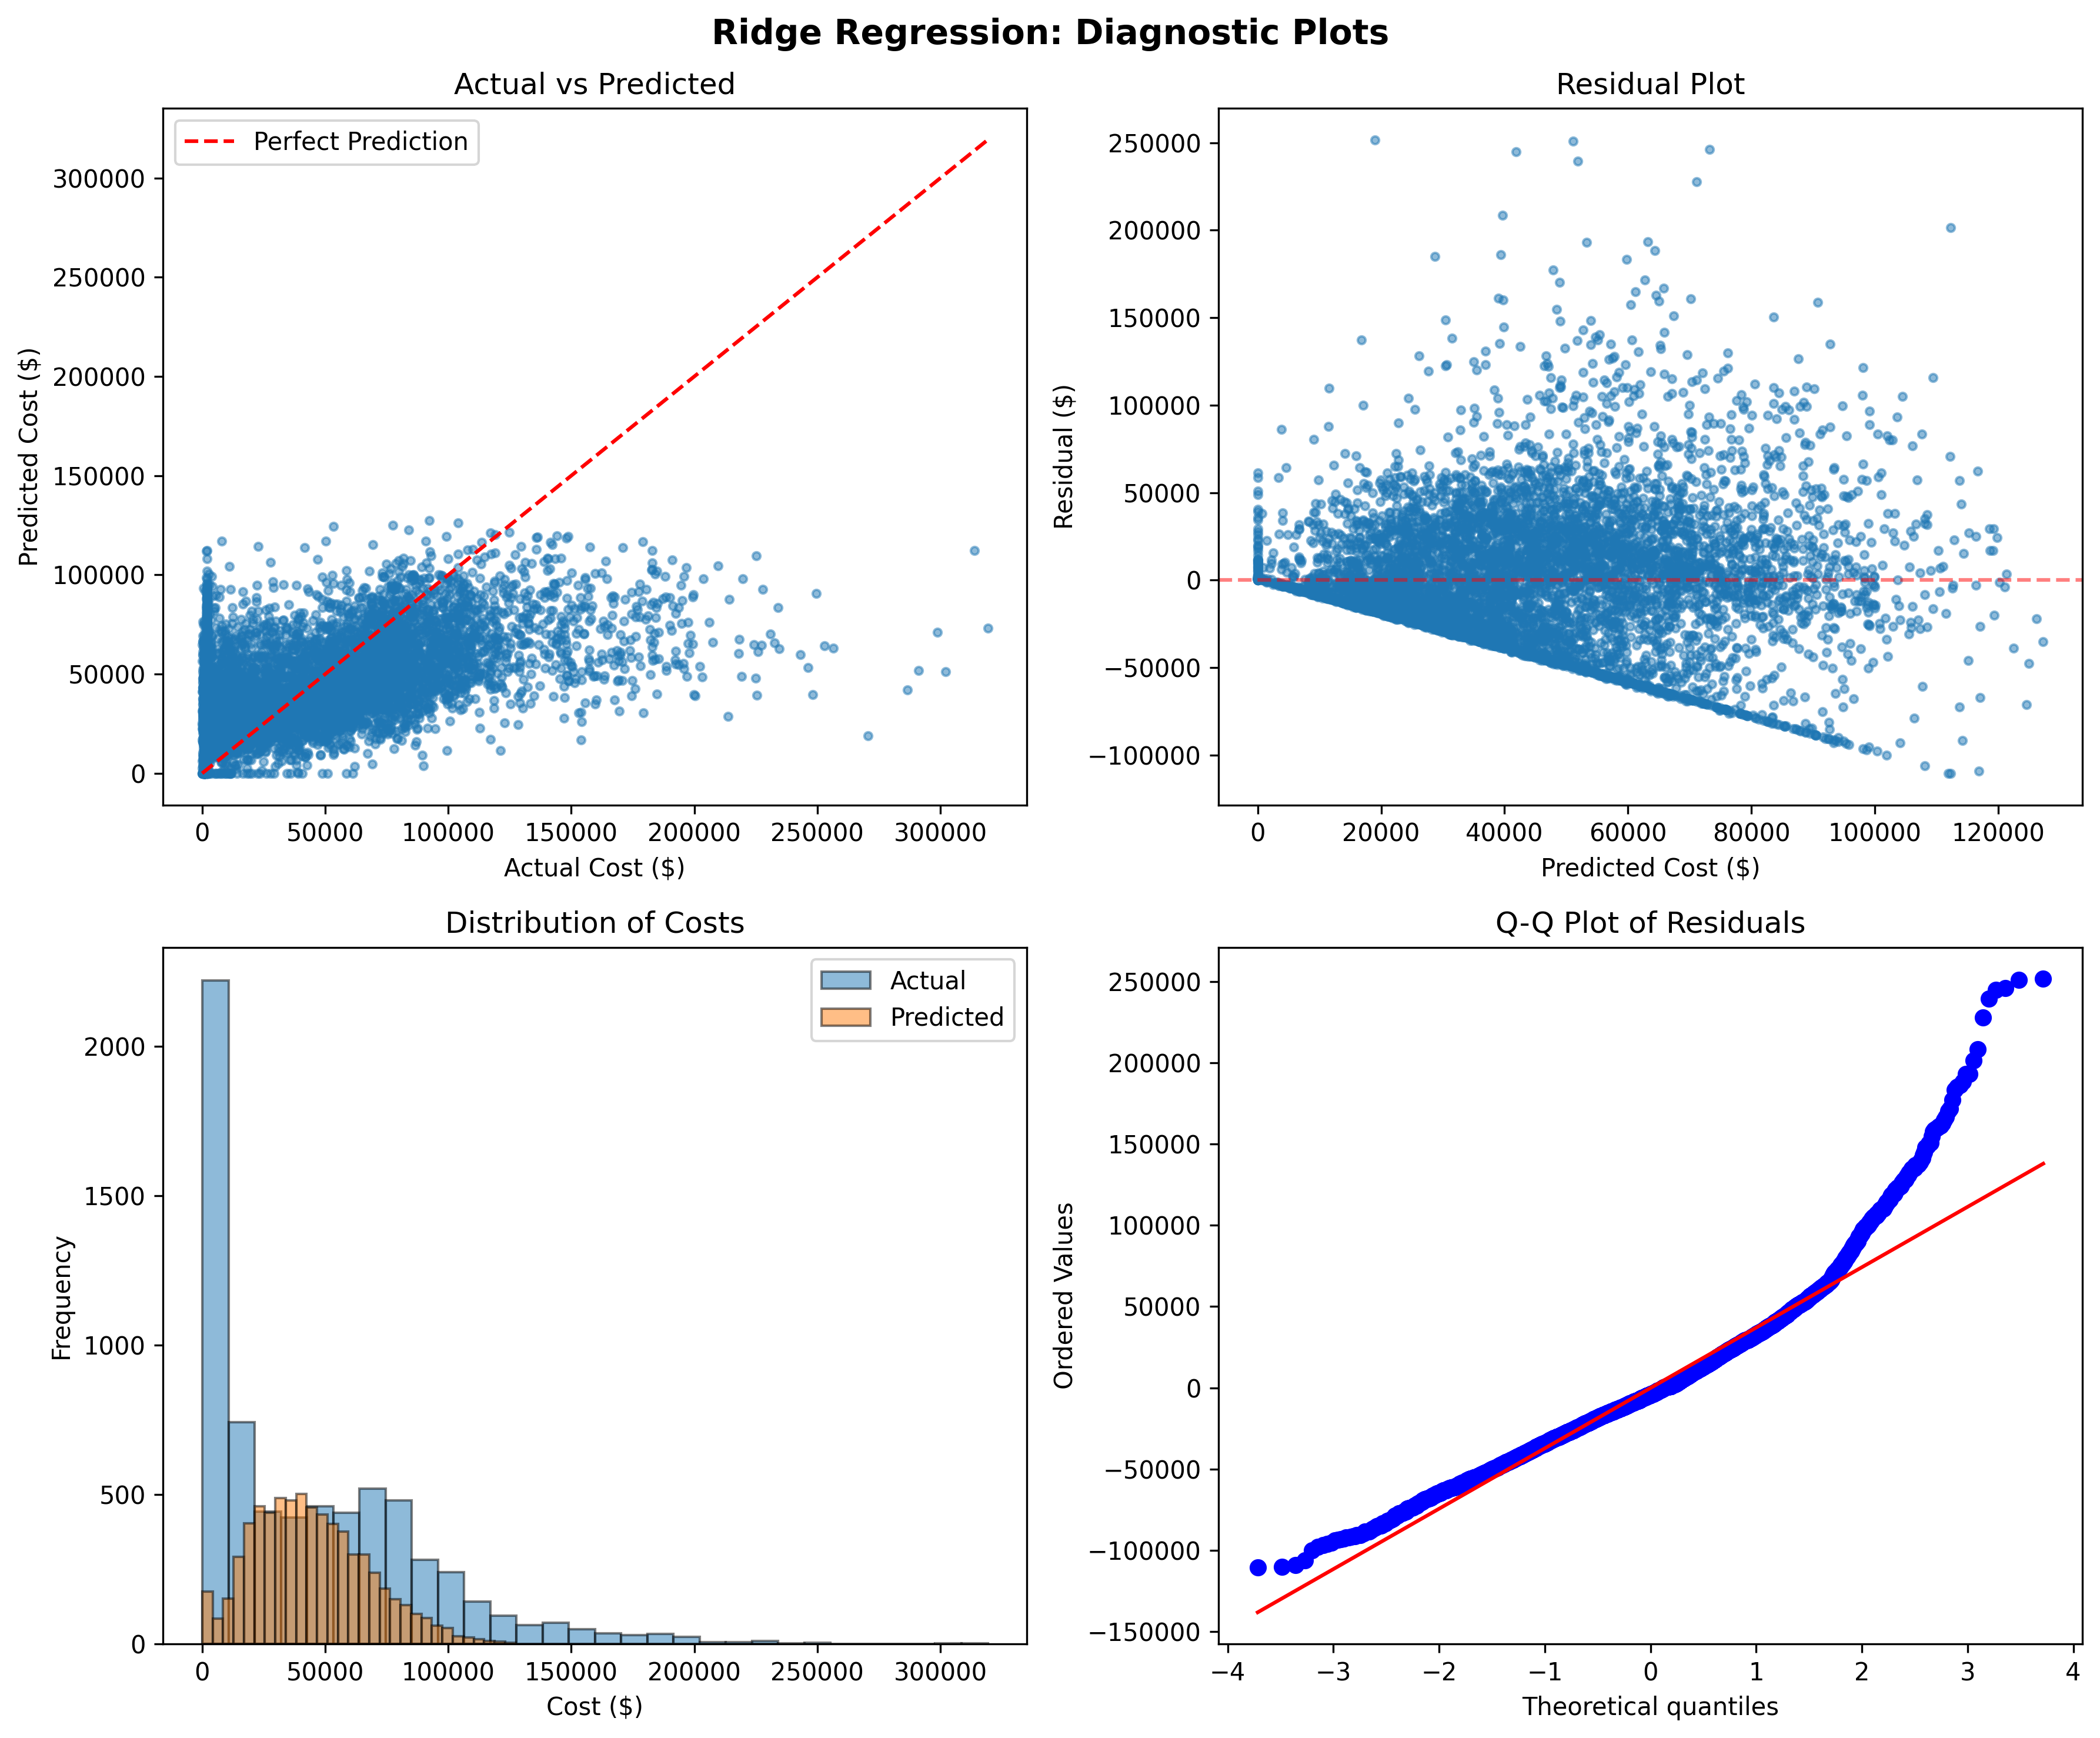
\includegraphics[width=\textwidth]{models/model_5/diagnostic_plots.png}
    \caption{Model 5 Ridge Diagnostic Plots -- Shows predicted vs actual, residuals, coefficient magnitudes, Q-Q plot, VIF analysis, and performance by cost quartile}
    \label{fig:model5_diagnostics}
\end{figure}

\begin{figure}[h]
    \centering
    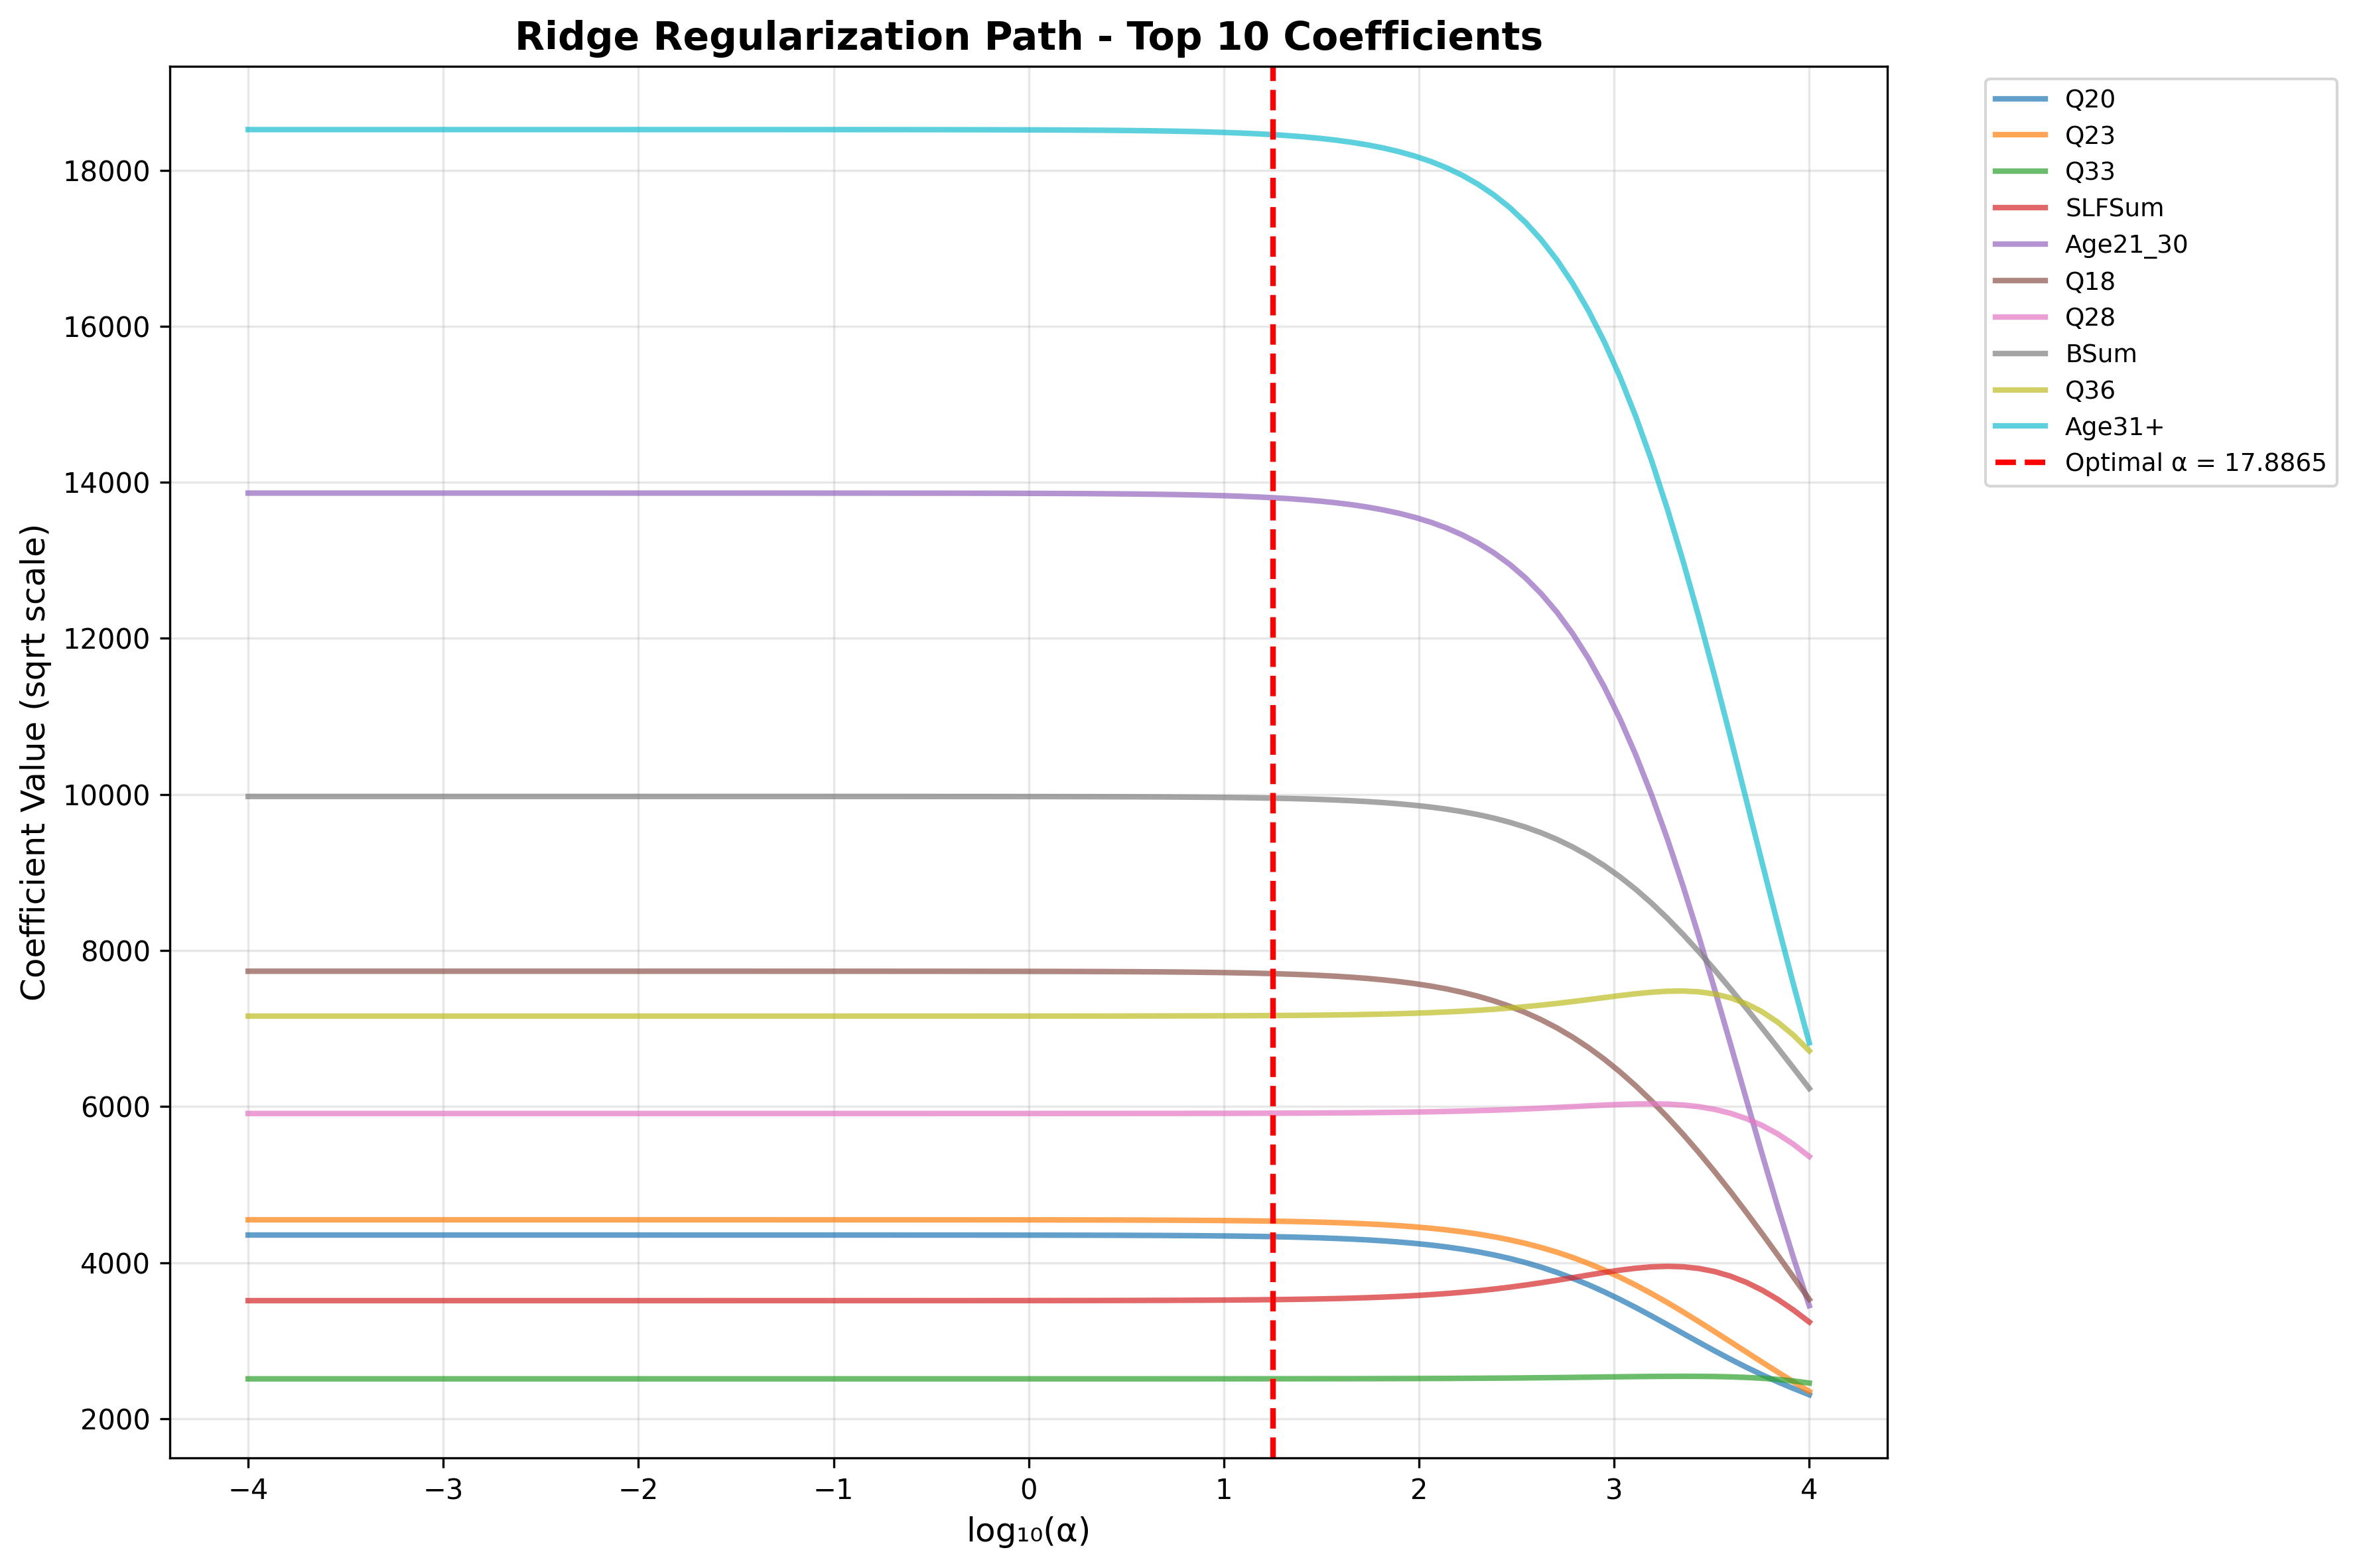
\includegraphics[width=\textwidth]{models/model_5/regularization_path.png}
    \caption{Ridge Regularization Path -- Shows coefficient shrinkage as $\lambda$ increases and cross-validation score optimization}
    \label{fig:model5_regpath}
\end{figure}

\section{Implementation Considerations}

\subsection{Technical Requirements}

\begin{itemize}
    \item \textbf{Software}: Standard implementation in R, Python, SAS, and other major packages
    \item \textbf{Computation Time}: $<$ 1 second with pre-computed $\lambda$
    \item \textbf{Memory Requirements}: Standard, similar to OLS
    \item \textbf{Database Integration}: Compatible with existing infrastructure
\end{itemize}

\subsection{Training and Documentation}

\begin{itemize}
    \item \textbf{Staff Training}: 8 hours on regularization concepts
    \item \textbf{Documentation}: Lambda selection process and interpretation
    \item \textbf{Pilot Testing}: 2,000 consumer comparison recommended
    \item \textbf{Rollout Timeline}: 12 months including education phase
\end{itemize}

\section{Advantages and Limitations}

\subsection{Advantages}

\begin{itemize}
    \item \textbf{Multicollinearity Management}: Effectively handles correlated predictors
    \item \textbf{Stability}: More stable coefficients than OLS
    \item \textbf{Generalization}: Better out-of-sample performance
    \item \textbf{No Feature Removal}: Retains all 22 predictors
    \item \textbf{Computational Efficiency}: Closed-form solution available
\end{itemize}

\subsection{Limitations}

\begin{itemize}
    \item \textbf{Interpretation Complexity}: Shrinkage concept may be difficult to explain
    \item \textbf{Parameter Tuning}: Requires cross-validation for $\lambda$ selection
    \item \textbf{Slight Accuracy Trade-off}: Minor reduction in R² for stability gain
    \item \textbf{Regulatory Concerns}: May face challenges in appeals due to complexity
\end{itemize}

\section{Risk Assessment}

\begin{table}[h]
\centering
\caption{Risk Matrix for Model 5 Ridge Implementation}
\begin{tabular}{p{3cm}ccp{5cm}}
\toprule
\textbf{Risk} & \textbf{Probability} & \textbf{Impact} & \textbf{Mitigation Strategy} \\
\midrule
Lambda misspecification & Low & Medium & Robust cross-validation protocol \\
Stakeholder confusion & High & Medium & Comprehensive training program \\
Regulatory challenge & Medium & High & Detailed documentation and justification \\
Technical implementation & Low & Low & Standard software packages available \\
\bottomrule
\end{tabular}
\end{table}

\section{Recommendation}

\subsection{Overall Assessment}

Model 5 Ridge regression offers a robust solution for managing multicollinearity while maintaining predictive accuracy. The \ModelFiveShrinkageFactor{}\% coefficient shrinkage provides stability without sacrificing interpretability, as all features remain in the model.

\subsection{Implementation Recommendation}

\textbf{Conditional Approval for Pilot Testing}

Recommend proceeding with:
\begin{enumerate}
    \item Parallel testing with current Model 5b for 6 months
    \item Educational workshops for stakeholders on regularization benefits
    \item Development of simplified explanations for regulatory compliance
    \item Quarterly monitoring of lambda stability and model performance
\end{enumerate}

\subsection{Success Metrics}

Monitor the following KPIs during pilot:
\begin{itemize}
    \item Maintain R² $>$ 0.79 on test data
    \item Condition number $<$ 15
    \item Maximum VIF $<$ 5
    \item Effective degrees of freedom between 15--20
    \item Stakeholder satisfaction $>$ 70\%
\end{itemize}

\section{Conclusion}

Model 5 Ridge regression represents a sophisticated enhancement to the current algorithm, offering improved stability and multicollinearity management at the cost of slightly increased complexity. The \ModelFiveRegularizationStrength{} regularization with $\lambda = $ \ModelFiveAlpha{} provides an optimal balance between bias and variance, making it suitable for production deployment following successful pilot testing and stakeholder education.

The model's ability to retain all 22 predictors while controlling their influence through shrinkage aligns with regulatory requirements for comprehensive assessment while addressing statistical concerns about predictor correlation. With proper implementation support and monitoring, Ridge regression can provide a more stable and generalizable budget allocation system.